\documentclass[11pt,a4paper]{article}
\usepackage[utf8]{vietnam}
\usepackage{amsmath,amssymb}
\usepackage{tabularx}
\usepackage{tikz}
\usepackage{xcolor}
\usepackage{fancyhdr}
\usepackage[top=1.8cm, bottom=2.0cm, left=1.8cm, right=1.8cm]{geometry}

\setlength{\parskip}{3pt}
\setlength{\parindent}{0pt}

\pagestyle{fancy}
\fancyhf{}
\renewcommand{\headrulewidth}{0.4pt}
\lhead{\footnotesize \textbf{CHÙA HƯƠNG SƠN -- ÔN THI VÀO 10}}
\rhead{\footnotesize \textbf{ĐỀ THI THỬ CUỐI HỌC KỲ I (ĐỀ SỐ 03)}}
\cfoot{\thepage}

\begin{document}

\noindent
\begin{tabular*}{\linewidth}{@{\extracolsep{\fill}}cc@{}}
\textbf{SỞ GIÁO DỤC VÀ ĐÀO TẠO} & \textbf{ĐỀ KIỂM TRA CUỐI HỌC KỲ I} \\
\textbf{CHÙA HƯƠNG SƠN} & \textbf{NĂM HỌC 2026 -- 2027} \\
\textbf{ĐỀ THI THỬ SỐ 03} & \textbf{MÔN: TOÁN -- LỚP 9} \\
\textit{(Đề thi gồm 03 trang)} & \textit{Thời gian làm bài: 90 phút (không kể thời gian phát đề)} \\
\end{tabular*}

\vspace{2mm}
\noindent
\rule{\linewidth}{0.8pt}

\vspace{1mm}
\noindent
Họ và tên thí sinh: \dotfill Số báo danh: \dotfill

\vspace{2mm}
\noindent
\textbf{\large I. TRẮC NGHIỆM KHÁCH QUAN (7,0 điểm)}

\vspace{1mm}
\noindent
\textbf{Phần 1. Trắc nghiệm nhiều lựa chọn (3,0 điểm).} \textit{Từ câu 1 đến câu 12, thí sinh chọn đáp án đúng nhất trong 4 đáp án A, B, C, D rồi ghi vào bài làm.}

\vspace{1.5mm}
\textbf{Câu 1.} Giá trị của biểu thức $\sqrt{45} - 2\sqrt{20} + \sqrt{5}$ bằng\\
\begin{tabularx}{\linewidth}{XXXX}
\textbf{A.} $0$. & \textbf{B.} $2\sqrt{5}$. & \textbf{C.} $-\sqrt{5}$. & \textbf{D.} $4\sqrt{5}$.
\end{tabularx}

\vspace{1.5mm}
\textbf{Câu 2.} Cho tam giác $ABC$ vuông tại $A$, có góc nhọn $\widehat{B} = \beta$. Khẳng định nào sau đây là đúng?\\
\begin{tabularx}{\linewidth}{XXXX}
\textbf{A.} $\cot \beta = \dfrac{AB}{AC}$. & \textbf{B.} $\sin \beta = \dfrac{AB}{BC}$. & \textbf{C.} $\cos \beta = \dfrac{AC}{BC}$. & \textbf{D.} $\tan \beta = \dfrac{AB}{AC}$.
\end{tabularx}

\vspace{1.5mm}
\textbf{Câu 3.} Bất phương trình nào sau đây là bất phương trình bậc nhất một ẩn?\\
\begin{tabularx}{\linewidth}{XXXX}
\textbf{A.} $5x - 15 \le 0$. & \textbf{B.} $0x - 4 > 0$. & \textbf{C.} $x^2 + 1 > 0$. & \textbf{D.} $\dfrac{3}{x} - 2 \le 0$.
\end{tabularx}

\vspace{1.5mm}
\textbf{Câu 4.} Cho $m < n$. Bất đẳng thức nào sau đây luôn đúng?\\
\begin{tabularx}{\linewidth}{XXXX}
\textbf{A.} $4m - 1 < 4n - 1$. & \textbf{B.} $-5m < -5n$. & \textbf{C.} $m + 2 > n + 2$. & \textbf{D.} $3 - m < 3 - n$.
\end{tabularx}

\vspace{1.5mm}
\textbf{Câu 5.} Căn bậc hai số học của số 144 là\\
\begin{tabularx}{\linewidth}{XXXX}
\textbf{A.} $12$ và $-12$. & \textbf{B.} $12$. & \textbf{C.} $-12$. & \textbf{D.} $72$.
\end{tabularx}

\vspace{1.5mm}
\textbf{Câu 6.} Điều kiện xác định của căn thức $\sqrt{15 - 5x}$ là\\
\begin{tabularx}{\linewidth}{XXXX}
\textbf{A.} $x \le 3$. & \textbf{B.} $x \ge 3$. & \textbf{C.} $x < 3$. & \textbf{D.} $x > 3$.
\end{tabularx}

\vspace{1.5mm}
\textbf{Câu 7.} Với mọi số thực $x \ge 7$, giá trị của biểu thức $\sqrt{(x-7)^2}$ bằng\\
\begin{tabularx}{\linewidth}{XXXX}
\textbf{A.} $x - 7$. & \textbf{B.} $7 - x$. & \textbf{C.} $-(x-7)$. & \textbf{D.} $(x-7)^2$.
\end{tabularx}

\vspace{1.5mm}
\textbf{Câu 8.} Giá trị của biểu thức $\sqrt[3]{-343}$ bằng\\
\begin{tabularx}{\linewidth}{XXXX}
\textbf{A.} $-7$. & \textbf{B.} $7$. & \textbf{C.} $-49$. & \textbf{D.} $49$.
\end{tabularx}

\vspace{1.5mm}
\textbf{Câu 9.} Trong đường tròn $(O; R)$, công thức tính diện tích hình tròn bán kính $R$ là\\
\begin{tabularx}{\linewidth}{XXXX}
\textbf{A.} $S = \pi R^2$. & \textbf{B.} $S = 2\pi R$. & \textbf{C.} $S = 2\pi R^2$. & \textbf{D.} $S = \pi R$.
\end{tabularx}

\vspace{1.5mm}
\textbf{Câu 10.} Cho đường tròn $(O; 6\text{ cm})$ và đường thẳng $\Delta$. Biết khoảng cách từ $O$ đến $\Delta$ là $6\text{ cm}$. Vị trí tương đối của đường thẳng $\Delta$ và đường tròn $(O)$ là\\
\begin{tabularx}{\linewidth}{XXXX}
\textbf{A.} Tiếp xúc nhau. & \textbf{B.} Cắt nhau. & \textbf{C.} Không giao nhau. & \textbf{D.} Trùng nhau.
\end{tabularx}

\vspace{1.5mm}
\textbf{Câu 11.} Cho hai đường tròn $(O; 9\text{ cm})$ và $(O'; 4\text{ cm})$. Biết khoảng cách giữa hai tâm $OO' = 5\text{ cm}$. Vị trí tương đối của hai đường tròn $(O)$ và $(O')$ là\\
\begin{tabularx}{\linewidth}{XXXX}
\textbf{A.} Tiếp xúc trong. & \textbf{B.} Tiếp xúc ngoài. & \textbf{C.} Cắt nhau. & \textbf{D.} Đựng nhau.
\end{tabularx}

\vspace{1.5mm}
\textbf{Câu 12.} Trên đường tròn $(O)$, cho góc ở tâm $\widehat{AOB} = 50^\circ$. Số đo của cung lớn $AB$ bằng\\
\begin{tabularx}{\linewidth}{XXXX}
\textbf{A.} $310^\circ$. & \textbf{B.} $130^\circ$. & \textbf{C.} $50^\circ$. & \textbf{D.} $100^\circ$.
\end{tabularx}

\vspace{3mm}
\noindent
\textbf{Phần 2. Trắc nghiệm Đúng -- Sai (2,0 điểm).} \textit{Trong mỗi ý a), b), c), d) ở câu 13 và câu 14, thí sinh chọn đúng hoặc sai và ghi chữ ``Đ'' hoặc ``S'' vào bài làm.}

\vspace{1.5mm}
\textbf{Câu 13.} Xét bài toán thực tế: ``Hai tổ công nhân cùng làm chung một đoạn đường bê tông nông thôn thì hoàn thành trong $12$ ngày. Nếu tổ 1 làm riêng trong $4$ ngày rồi tổ 2 đến làm tiếp trong $10$ ngày nữa thì cả hai tổ hoàn thành được đúng $\dfrac{1}{2}$ công việc. Gọi thời gian tổ 1 và tổ 2 làm một mình hoàn thành toàn bộ công việc lần lượt là $x$ và $y$ (ngày, $x, y > 12$).''\\
Xét tính đúng sai của các khẳng định sau:
\begin{center}
\begin{tabularx}{\linewidth}{|X|c|c|}
\hline
\textbf{Khẳng định} & \textbf{Đúng} & \textbf{Sai} \\
\hline
a) Trong 1 ngày, cả hai tổ cùng làm được $\dfrac{1}{12}$ khối lượng công việc. & & \\
\hline
b) Khi tổ 1 làm 4 ngày và tổ 2 làm 10 ngày, phương trình biểu thị là: $\dfrac{4}{x} + \dfrac{10}{y} = 1$. & & \\
\hline
c) Hệ phương trình xác định thời gian $x$ và $y$ là: $\begin{cases} \dfrac{1}{x} + \dfrac{1}{y} = \dfrac{1}{12} \\ \dfrac{4}{x} + \dfrac{10}{y} = \dfrac{1}{2} \end{cases}$. & & \\
\hline
d) Nếu làm một mình, tổ 1 hoàn thành trong $20$ ngày, tổ 2 hoàn thành trong $30$ ngày. & & \\
\hline
\end{tabularx}
\end{center}

\vspace{2mm}
\textbf{Câu 14.} Cho đường tròn $(O; 10\text{ cm})$, đường kính $AB$ vuông góc với dây cung $CD$ tại điểm $H$ ($H$ nằm giữa $O$ và $B$). Biết độ dài dây cung $CD = 16\text{ cm}$.\\
Xét tính đúng sai của các khẳng định sau:
\begin{center}
\begin{tabularx}{\linewidth}{|X|c|c|}
\hline
\textbf{Khẳng định} & \textbf{Đúng} & \textbf{Sai} \\
\hline
a) Điểm $H$ là trung điểm của dây cung $CD$ và $HC = 8\text{ cm}$. & & \\
\hline
b) Khoảng cách từ tâm $O$ đến dây cung $CD$ là $OH = 6\text{ cm}$. & & \\
\hline
c) Độ dài đoạn thẳng $HB$ bằng $4\text{ cm}$. & & \\
\hline
d) Chu vi tam giác $ACD$ bằng $48\text{ cm}$. & & \\
\hline
\end{tabularx}
\end{center}

\vspace{3mm}
\noindent
\textbf{Phần 3. Trắc nghiệm trả lời ngắn (2,0 điểm).} \textit{Từ câu 15 đến câu 18, thí sinh chỉ ghi kết quả cuối cùng vào bài làm.}

\vspace{1.5mm}
\textbf{Câu 15.} Nghiệm của bất phương trình $4(x - 2) + 3 > 5(x + 1) - 8$ là $\dots\dots\dots$

\vspace{1.5mm}
\textbf{Câu 16.} Giá trị của biểu thức $P = \sqrt{(\sqrt{6} - 3)^2} + \sqrt{6}$ bằng $\dots\dots\dots$

\vspace{1.5mm}
\noindent
\begin{minipage}[c]{0.65\linewidth}
\textbf{Câu 17.} Để đo chiều rộng $AB$ của một khúc sông mà không cần bơi qua bờ bên kia, một người đứng tại vị trí $C$ cùng bờ với $B$ sao cho tam giác $ABC$ vuông tại $B$. Người đó đo được khoảng cách $BC = 40\text{ m}$ và dùng giác kế ngắm được góc $\widehat{ACB} = 36^\circ$ (xem hình vẽ bên). Tính chiều rộng $AB$ của khúc sông (làm tròn kết quả đến chữ số thập phân thứ hai của mét).
\end{minipage}\hfill
\begin{minipage}[c]{0.32\linewidth}
\centering
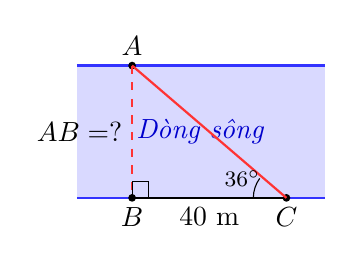
\begin{tikzpicture}[scale=0.7]
  % Dòng sông
  \fill[blue!15] (0,0) rectangle (4.5,2.4);
  \draw[thick, blue!80] (0,0) -- (4.5,0);
  \draw[thick, blue!80] (0,2.4) -- (4.5,2.4);
  \node[blue!80!black] at (2.25, 1.2) {\textit{Dòng sông}};
  % Các điểm
  \coordinate (A) at (1.0, 2.4);
  \coordinate (B) at (1.0, 0);
  \coordinate (C) at (3.8, 0);
  \fill (A) circle (2pt) node[above] {$A$};
  \fill (B) circle (2pt) node[below] {$B$};
  \fill (C) circle (2pt) node[below] {$C$};
  \draw[dashed, thick, red!80] (A) -- (B);
  \draw[thick] (B) -- (C);
  \draw[thick, red!80] (A) -- (C);
  \draw (1.0, 0) rectangle (1.3, 0.3);
  \draw (3.8, 0) ++(180:0.6) arc (180:144:0.6);
  \node at (3.0, 0.35) {\footnotesize $36^\circ$};
  \node[below] at (2.4, 0) {$40\text{ m}$};
  \node[left] at (1.0, 1.2) {$AB = ?$};
\end{tikzpicture}
\end{minipage}

\vspace{1.5mm}
\textbf{Câu 18.} Một hình quạt tròn có bán kính $R = 15\text{ cm}$ và góc ở tâm tương ứng là $150^\circ$. Tính diện tích của hình quạt tròn đó (lấy $\pi \approx 3{,}14$, làm tròn kết quả đến hàng phần mười, đơn vị: $\text{cm}^2$).

\vspace{4mm}
\noindent
\textbf{\large II. TỰ LUẬN (3,0 điểm).} \textit{Thí sinh trình bày lời giải chi tiết vào tờ giấy thi.}

\vspace{2mm}
\textbf{Câu 19 (1,0 điểm).}
\begin{itemize}
  \item[a)] \textit{(0,5 điểm)} Giải hệ phương trình: $\begin{cases} 4x + 3y = 11 \\ 3x - y = 5 \end{cases}$.
  \item[b)] \textit{(0,5 điểm)} Cho biểu thức $P = \left( \dfrac{\sqrt{x}}{\sqrt{x}+1} - \dfrac{1}{x+\sqrt{x}} \right) : \dfrac{\sqrt{x}-1}{x}$ với $x > 0, x \ne 1$. Rút gọn biểu thức $P$.
\end{itemize}

\vspace{2mm}
\textbf{Câu 20 (1,5 điểm).} Cho đường tròn $(O; R)$ và điểm $M$ nằm ngoài đường tròn. Từ $M$ kẻ hai tiếp tuyến $MA, MB$ với đường tròn $(O)$ ($A, B$ là các tiếp điểm). Kẻ cát tuyến $MCD$ không đi qua tâm $O$ ($C$ nằm giữa $M$ và $D$).
\begin{itemize}
  \item[a)] \textit{(0,75 điểm)} Chứng minh rằng bốn điểm $M, A, O, B$ cùng thuộc một đường tròn và $OM \perp AB$.
  \item[b)] \textit{(0,75 điểm)} Chứng minh rằng: $MA^2 = MC \cdot MD$.
\end{itemize}

\vspace{2mm}
\textbf{Câu 21 (0,5 điểm).}
\begin{itemize}
  \item[a)] \textit{(0,25 điểm)} Một người nông dân dùng một đoạn lưới thép B40 dài $40\text{ m}$ để rào thành một khu đất hình chữ nhật trồng rau sạch tựa lưng vào một bức tường đá thẳng có sẵn (không cần rào phía tường đá). Hãy xác định các kích thước của khu đất để diện tích trồng rau đạt giá trị lớn nhất.
  \item[b)] \textit{(0,25 điểm)} Cho ba số thực dương $a, b, c$ thỏa mãn $a + b + c \le 3$. Tìm giá trị nhỏ nhất của biểu thức:
  \[
  Q = a + b + c + \dfrac{1}{a} + \dfrac{1}{b} + \dfrac{1}{c}.
  \]
\end{itemize}

\vspace{4mm}
\begin{center}
\textbf{---------- HẾT ----------}\\
\textit{(Cán bộ coi thi không giải thích gì thêm)}
\end{center}

\end{document}
